\section{Overview}
    % Problems with Existing Systems
    \subsection{Need for a New Benchmark}
    Traditionally, these systems have been evaluated over small manually curated gold datasets (e.g., \cite{ReVerb1, Ollie}). There are two problems with this approach. One, it is not reliable due to the small size of annotation. Second, it lacks standardization, since there is no single gold dataset over which all systems are evaluated. Moreover, the guidelines to annotate may vary across datasets and annotators. Recently, some standard benchmarks datasets and evaluators have been proposed: OIE2016 \citep{OIE2016}, RelVis \citep{Relvis}, and  Wire57 \citep{Wire57}. Unfortunately, these datasets are either too small or too noisy to meaningfully compare Open IE systems. 

    % CaRB intro
    \subsection{Establishing a new State-of-the-Art}
    In response, we propose a new benchmark system CaRB:  \textbf{C}rowdsourced \textbf{a}utomatic open \textbf{R}elation extraction \textbf{B}enchmark \citep{bhardwaj&al19}, which has a good sized and high quality dataset, along with better evaluation metrics. In order to create this gold dataset, we crowdsource human annotation of extractions using Amazon Mechanical Turk (MTurk) using the same original sentences as OIE2016. Our MTurk task has an automated system for training and qualifying workers, which makes crowdsourcing this annotation feasible.

    Two Open IE experts (authors of this paper) manually annotate 50 random sentences, which are then used as expert ground truth to evaluate the respective tuples in OIE2016's and CaRB's gold datasets  (Tables \ref{tab:token-level},\ref{tab:lexical}). We find that CaRB outperforms OIE2016 by 21 points in precision and 16 points in recall in token level match. This demonstrates that CaRB's gold dataset is significantly more accurate than OIE2016's. Additionally, when evaluating all systems using our benchmark, we notice that CaRB reverses OIE2016's ranking of PropS and ClausIE. Human verification, again through crowdsourcing, verifies that two systems are ranked more accurately by CaRB. We release CaRB's dataset, along with its evaluator as a novel benchmark for further use by research community.\footnote{\texttt{\href{https://github.com/dair-iitd/CaRB}{https://github.com/dair-iitd/CaRB}}}


\section{Crowdsourcing CaRB Dataset}

    To overcome the shortcomings of dataset noise and size, we crowdsource a high-quality gold dataset for Open IE. We ask  workers over Amazon Mechanical Turk (MTurk) to annotate extractions for the 1,282 sentences in dev and test splits of OIE2016. The workers annotate tuples in the form (arg1, rel, arg2), and also annotate location and time attributes for each tuple, when possible. 

    Open IE annotations are not easy to obtain from non-expert workers. To get acceptable quality,  we train workers using a tutorial that doubles up as a qualification test. Their performance in the test is automatically graded. Only workers that pass this are allowed to move on to the main task. The qualification is integrated with the task so that a new worker is served the tutorial and test first, but a qualified worker is directly taken to the main task. This makes the crowdsourcing process scalable. 

    We divide the task of annotating a sentence into three steps: (1) identifying the relation, (2) identifying the arguments for that relation, and (3) optionally identifying the location and time attributes for the tuple.  The training process for the annotators is split into four steps,  each of which focuses on a different guideline for Open IE. These are:

    \begin{enumerate}%[noitemsep]
        \item {\bf Completeness:} The worker must attempt to extract {\em all} assertions from the sentence.
        \item {\bf Assertedness:} Each tuple must be implied by the original sentence.
        \item {\bf Informativeness:} The worker must include the maximum amount of relevant information in an argument.
        \item {\bf Atomicity:} Each tuple must be an indivisible unit. Whenever possible, the worker must extract multiple atomic tuples from a sentence that has conjunctions. 
    \end{enumerate}
    
    We also develop a user-friendly interface for annotating the sentences, which almost eliminates the need for workers to type anything. 
    However, we note that several workers got frustrated in our qualification test, could not understand the task and left the job. However, several good workers completed the task successfully, and annotated significant high-quality data for us.
    
    For sentences involving reporting verbs like {\em said, told, asked,} etc., some systems annotate additional attributional context for every utterance \cite{Ollie}. For this, we create a separate task, so as to prevent workers from being bombarded with all the rules at the same time.

    We post-process the data to remove obvious incorrect annotations, like ones with a missing arg1 or rel. We also follow the convention of ending a relation with a preposition instead of beginning arg2 with one, so all prepositions are shifted to rel.

\section{The CaRB Scorer}

    We now describe CaRB's approach for scoring system predictions against the gold. Instead of greedily matching gold tuples to system tuples in arbitrary order, CaRB creates an all-pair matching table, with each column as system tuple and each row as gold tuple. It computes precision and recall scores between each pair of tuples. Then, for computing overall recall, the maximum recall score is taken in each row, and averaged. By taking the maximum, recall computation matches a gold tuple with the closest system extraction. For computing precision, the system predictions are matched one to one with gold tuples, in the order of best match score to worst. The match precision scores are then averaged to compute precision.  To compute precision-recall curve this computation is done at different confidence thresholds of system extractions.

    \begin{table}[h]
        {\small
        \centering
        \begin{tabular}{|l|l|l|l|} 
        \hline
        Sentence & \begin{tabular}[c]{@{}l@{}}{\em I ate an apple}\\ {\em and an orange.}\end{tabular}         & \multicolumn{1}{l}{(prec,rec)} &           \\ 
        \hline
        Gold     & \begin{tabular}[c]{@{}l@{}}(I; ate; an apple)\\(I; ate; an orange)\end{tabular} & OIE2016                        & CaRB      \\ 
        \hline
        System 1 & \begin{tabular}[c]{@{}l@{}}(I; ate; an apple\\ and an orange)\end{tabular}      & (1,0.5)                        & (0.57,1)  \\ 
        \hline
        System 2 & (I; ate; an apple)                                                              & (1,0.5)                        & (1,0.87)  \\
        \hline
        \end{tabular}
        \caption{One-to-One Match vs. Multi Match}
        \label{tab:one2one_vs_multi_match}
        }
    \end{table}

    In this way, CaRB's recall computation uses the notion of {\em multi-match}, wherein a gold tuple can match multiple system extractions. This is helpful in avoiding penalizing a system very heavily if it stuffs information from multiple gold tuples in a single extraction. Table \ref{tab:one2one_vs_multi_match} displays an example wherein system 1 combines information from two gold tuples in a single extraction, and system 2 only extracts one of the gold tuples. One-to-one match (OIE2016) is indifferent between the two which means that for OIE2016, adding more information in the same extraction has no value at all. However, multi match (CaRB) assigns higher recall to system 1, since it contains strictly more information, and higher precision to system 2, since its prediction exactly matched a gold extraction. 

    On the other hand, CaRB uses {\em single match} for precision. This is because CaRB’s gold tuples are atomic, and cannot be further divided into more tuples. By single matching for precision, CaRB penalizes Open IE systems that produce several very similar and redundant extractions.

    Another significant change from OIE2016 scorer is in the use of {\em tuple match} instead of {\em lexical match}. CaRB matches relation with relation, and arguments with arguments, however OIE2016 serialized the tuples into a sentence and just computed lexical matches. 
    
    \begin{table}[h]
        \centering
        {\small
        \begin{tabular}{|l|l|l|l|} 
        \hline
        Sentence & {\em I ate an apple.}    & \multicolumn{1}{l}{(prec,rec)} &        \\ 
        \hline
        Gold     & (I; ate; an apple) & OIE2016                        & CaRB   \\ 
        \hline
        System 1 & (I; ate; an apple) & (1,1)                          & (1,1)  \\ 
        \hline
        System 2 & (ate; an apple; I) & (1,1)                          & (0,0)  \\
        \hline
        \end{tabular}
        \caption{Tuple Match vs. Lexical Match}
        \label{tab:tuple_vs_lexical_match}
        }
        \vspace*{-2ex}
    \end{table}

    Table \ref{tab:tuple_vs_lexical_match} illustrates an example when the arguments are shuffled, lexical match (OIE2016) shows no effect but tuple match (CaRB) rightfully decreases the scores. To avoid spurious matches, CaRB considers only matches with atleast one common word in the relation field.

    Finally, some Open IE systems extract n-ary tuples and others do not. To treat all systems on equal footing, we follow previous work and append all higher numbered arguments into arg2. 

\section{Evaluation}
    \subsection{Dataset Quality}

        We first estimate the overall quality of the crowdsourced dataset. To this end, two authors of this paper annotate 50 dev sentences from OIE2016 to create an expert dataset. They first independently annotate tuples from these sentences, achieving an agreement F1 score of 83. They then resolve the differences and  merge these independent sets. This is taken as an expert gold against which both OIE2016 and CaRB datasets are assessed. 

        \begin{table}[h!]
        \centering
        \begin{tabular}{|c|c|c|c|}
        \hline
        Dataset       & Precision & Recall & F1    \\ \hline
        OIE2016 & 0.65     & 0.55  & 0.60 \\ %\hline
        CaRB         & 0.87     & 0.71  & 0.78 \\ \hline
        \end{tabular}
        \vspace*{-1ex}
        \caption{Data quality using token-level match}
        \label{tab:token-level}
        \end{table}
        
        \begin{table}[h]
        \vspace*{-1ex}
        \centering
        \begin{tabular}{|c|c|c|c|}
        \hline
                & Precision & Recall & F1   \\ \hline
        OIE2016 & 0.67      & 0.51      & 0.57 \\ %\hline
        CaRB   & 0.74      & 0.73      & 0.73 \\ \hline
        \end{tabular}
        \vspace*{-1ex}
        \caption{Data quality using lexical match}
        \label{tab:lexical}
        \vspace*{-1ex}
        \end{table}
        
        % OIE2016 Gold vs CaRB Gold
        \begin{table*}[t!]
            \centering
            \begin{tabular}{|l|l|} 
            \hline
            Sent. \# 1 & \textit{ Butters Drive in the Canberra suburb of Phillip is named in his honour . }                                                                                                                                                                                                                                                                                                                         \\ 
            \hline
            OIE2016    & \begin{tabular}[c]{@{}l@{}}( in the Canberra suburb of Phillip is named in his honour . ; drive; ),\\ ( Butters Drive in the Canberra suburb of Phillip ; named ; his honour ) \end{tabular}                                                                                                                                                                                                                \\ 
            \hline
            CaRB       & \begin{tabular}[c]{@{}l@{}}( Butters Drive in the Canberra suburb of Phillip ; is named ; in his honour),\\( Butters Drive ; is ; in the Canberra suburb of Phillip ) \end{tabular}                                                                                                                                                                                                                         \\ 
            \hhline{|==|}
            Sent. \# 2 & \begin{tabular}[c]{@{}l@{}}\textit{ It was only incidentally that economic issues appeared in nationalist}\\\textit{political forms . }\end{tabular}                                                                                                                                                                                                                                                        \\ 
            \hline
            OIE2016    & ( incidentally ; appeared ; economic issues ; nationalist political forms . )                                                                                                                                                                                                                                                                                                                               \\ 
            \hline
            CaRB       & (economic issues ; appeared only incidentally in ; nationalist political forms)                                                                                                                                                                                                                                                                                                                             \\ 
            \hhline{|==|}
            Sent. \# 3 & \begin{tabular}[c]{@{}l@{}}																		\textit{The main reason for this adoption over mainline gimp was its support for }\\\textit{high bit depths which can be~required for film work . }\end{tabular}                                                                                                                                                                                               \\ 
            \hline
            OIE2016    & ( high bit depths ; required ; film work )                                                                                                                                                                                                                                                                                                                                                                  \\ 
            \hline
            CaRB       & \begin{tabular}[c]{@{}l@{}}( this adoption ; has support for ; high bit depths ),\\( high bit depths ; can be required for ; film work ),\\ ( this adoption ; was over ; mainline gimp ),\\( mainline gimp ; has no support for ; high bit depths ),\\ ( its support for high bit depths which can be required for film work ;\\was The main reason for ; this adoption over mainline gimp ) \end{tabular}  \\ 
            \hhline{|==|}
            Sent. \# 4 & \begin{tabular}[c]{@{}l@{}}																		\textit{The number of ones equals the number of zeros plus one , since the state }\\\textit{containing only zeros can not occur .~}									 \end{tabular}                                                                                                                                                                                                     \\ 
            \hline
            OIE2016    & \begin{tabular}[c]{@{}l@{}}( The number of ones ; equals ; the number of zeros plus one ; \\since the state containing only zeros can not occur ),\\( the state ; containing ; only zeros ),\\( the state containing only zeros ; occur ) \end{tabular}                                                                                                                                                     \\ 
            \hline
            CaRB       & \begin{tabular}[c]{@{}l@{}}( The number of ones ; equals ; the number of zeros plus one ),\\ ( the state containing only zeros ; can not occur ) \end{tabular}                                                                                                                                                                                                                                              \\
            \hline
            \end{tabular}
            \caption{Sample gold annotations for OIE2016 vs. CaRB}
            \label{tab:gold_example}
        \end{table*}

        Tables  \ref{tab:token-level} and \ref{tab:lexical} estimate dataset quality of OIE2016 and CaRB. We find that CaRB has enormously high precision and recall values, suggesting that it is a much cleaner dataset. Table \ref{tab:gold_example} compares the crowd sourced annotations and OIE2016 gold annotations for some sample sentences. While there is still scope for improvement, CaRB dataset appears much better than the OIE2016's gold.

        \citet{OIE2016} remark that their gold dataset reaches an F1 of 95.8 on their expert annotation, whereas our assessment suggest values around 60. We surmise that this discrepancy is due to the different gold-prediction scoring schemes used. In original OIE2016 paper, the authors ``match an automated extraction with a gold proposition if both agree on the grammatical head of all of their elements (predicate and arguments)".\footnote{This scheme is later changed in their github  repository to a lexical match, where if the fraction of words in the prediction also present in the gold is above a threshold, the pair is declared a match.} The head match criterion is a much laxer scheme than ours and can explain the very high F1 score against their expert annotation.

    \subsection{Comparison of Open IE Systems}
        % Performance of OpenIE systems on CaRB
        \begin{table}[h!]
        %\vspace*{-1ex}
        \centering
        \begin{tabular}{|l|c|c|c|c|}
        \hline
        System  & Precision & Recall & F1 & AUC  \\ \hline
        % Stanford & {\bf 0.73}      & 0.28      & 0.41 & 0.24 \\ %\hline
        % Ollie       & 0.575          & 0.391          & 0.465 & 0.272 \\ %\hline
        % PropS       & 0.492          & 0.556          & 0.522 & 0.310 \\ %\hline
        % OpenIE 4    & {\bf 0.618}    & 0.515          & \bf{0.562} & \bf{0.351}\\ %\hline
        % OpenIE 5    & 0.604          & 0.521          & 0.559 & 0.349\\ %\hline
        % ClausIE     & 0.508          & \bf{0.593}     & 0.548 & 0.340\\ \hline
        
        Ollie       & 0.505          & 0.346          & 0.411 & 0.224 \\ %\hline
        PropS       & 0.340          & 0.300          & 0.319 & 0.126 \\ %\hline
        OpenIE 4    & {\bf 0.553}    & 0.437          & \bf{0.488} & \bf{0.272}\\ %\hline
        OpenIE 5    & 0.521          & 0.424          & 0.467 & 0.245\\ %\hline
        ClausIE     & 0.411          & \bf{0.496}     & 0.450 & 0.224\\ \hline
        \end{tabular}
        \vspace*{-1ex}
        \caption{Performance of Open IE systems on CaRB}
        \vspace*{-2ex}
        \label{tab:carb}
        \end{table}

        We test the different Open IE systems depicted in \citet{OIE2016}, using the CaRB dataset and scorer. The p-r curves obtained using OIE2016 and CaRB are outlined in figures \ref{fig:pr_oie16} (reproduced from \citet{Rnnoie}) and \ref{fig:pr_carb}. Precision, recall and F1 scores (at max F1 point) and area under precision-recall curve are reported in Table \ref{tab:carb}. It can be seen that the curve for PropS lies above ClausIE at all times in OIE2016, but PropS performs the worse of all systems in CaRB. To verify that CaRB indeed gives the correct ranking, we turn back to human verification.

        % PR_oie16
        \begin{figure}[h!]
            \centering
        %   \includegraphics[width=\linewidth]{gabi.PNG}
        \vspace*{-2ex}
            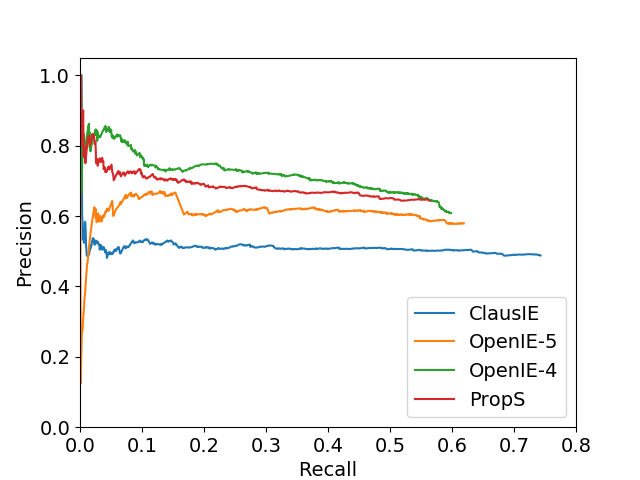
\includegraphics[width=0.7\columnwidth]{images/carb/oie16.png}
            \caption{Comparison of Open IE systems using OIE2016}
            \label{fig:pr_oie16}
        \end{figure}
        
        % PR_carb
        \begin{figure}[h!]
            \centering
        \vspace*{-3ex}
        %   \includegraphics[width=\linewidth]{carb.PNG}
            \includegraphics[width=0.7\columnwidth]{images/carb/carb.png}
            \caption{Evaluation of Open IE systems using CaRB}
            \label{fig:pr_carb}
        \end{figure}

    
    \subsection{Human Verification}
        Through human verification, our goal is to learn the accurate ranking for ClausIE and PropS.  We randomly select 100 test sentences and evaluate both system extractions on this subset. 

        We assess the correct ranking between PropS and ClausIE using MTurk. Four workers are shown the extractions from both systems in random order and asked to either choose one of the systems as the better one or indicate that both are equal. The majority opinion of these four is considered as the correct ranking for that sentence, an equal split leading to a tie. In this experiment, we only allow MTurk workers who have been trained for Open IE for the crowdsourcing task to participate.

        Of these 100 sentences, PropS is chosen to have performed better for 15, ClausIE for 69 whereas 16 ended up in a tie. ClausIE is indeed considered the better system in human evaluation, and we verify that CaRB gives an accurate ranking of these two systems compared to OIE2016. 

\section{Conclusion}
    We contribute CaRB \citep{bhardwaj&al19}, a crowdsourced dataset for evaluation and comparison of Open IE systems. We assess this dataset against an expert-annotated dataset and find that it is dramatically more accurate than the existing OIE2016 benchmark dataset. 

    We also implement a scorer that computes precision, recall and area under p-r curve for a given system output by matching it with the CaRB dataset. In designing our scorer, we make several design choices that deviate from prior work in both match scores and also in finding the best match for a tuple. We believe our scheme treats various systems fairly. And in one case where CaRB and OIE2016 give different rankings to two Open IE systems, we demonstrate via human evaluation that the ranking given by CaRB is the accurate one. We release the dataset and scorer for further use by research community. 

